% B and A are car-tail contact points on AB; icons extend right of each vertex.
% 2015_hubei_liberal_q15 tetrahedron schematic (application_diagram, schematic).
% D vertically above C; C-A dashed, others solid; highway + lower line + two car icons.
\usetikzlibrary{arrows.meta}
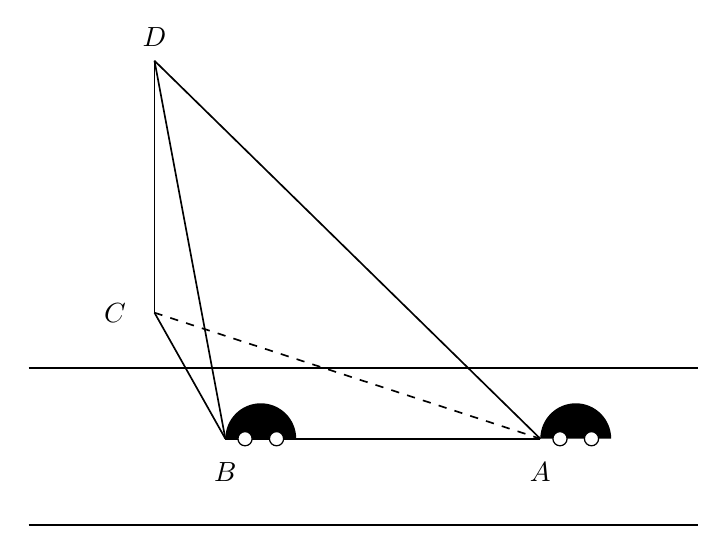
\begin{tikzpicture}[x=1cm,y=1cm,line width=.6pt,font=\normalsize,>=Stealth]
  % highway line above cars and lower parallel line
  \draw ( -2.5,0.9) -- (6.0,0.9);
  \draw (-2.5,-1.1) -- (6.0,-1.1);
  % road segment B-A at wheel level
  \draw (0,0) -- (4,0);
  % tetrahedron edges
  \draw (-0.9,1.6) -- (-0.9,4.8);
  \draw (-0.9,4.8) -- (0,0);
  \draw (-0.9,4.8) -- (4,0);
  \draw (-0.9,1.6) -- (0,0);
  \draw[dash pattern=on 3pt off 3pt] (-0.9,1.6) -- (4,0);
  % car icons: black half-discs with two white wheels
  \fill[black] (0,0) arc (180:0:0.45) -- cycle;
  \fill[white,draw=black,line width=.45pt] (0.25,0) circle (0.09);
  \fill[white,draw=black,line width=.45pt] (0.65,0) circle (0.09);
  \fill[black] (4,0) arc (180:0:0.45) -- cycle;
  \fill[white,draw=black,line width=.45pt] (4.25,0) circle (0.09);
  \fill[white,draw=black,line width=.45pt] (4.65,0) circle (0.09);
  % labels with clearance
  \node[inner sep=0pt] at (-0.9,5.1) {$D$};
  \node[inner sep=0pt] at (-1.4,1.6) {$C$};
  \node[inner sep=0pt] at (0,-0.42) {$B$};
  \node[inner sep=0pt] at (4,-0.42) {$A$};
\end{tikzpicture}
